\newpage % Rozdziały zaczynamy od nowej strony.
\cleardoublepage % Zaczynamy od nieparzystej strony
\pagestyle{headings}

\section{Wyniki i wnioski}

Celem pracy było zaprojektowanie, nauczenie i przetestowanie działania algorytmu Sztucznej Sieci Neurnonowej z użyciem 
układu FPGA oraz porównanie z rozwiązaniem programowym uruchamianym na komputerze PC. Podczas projektu powstało kilka modeli Sztucznej Sieci 
Neuronowej klasyfikującej odręcznie pisane cyfry. Aby porównać rozwiązanie, realizowane w technice HLS z implementacją przy użyciu pakietu \emph{keras}, każdy z modeli poddano testom, które zostały podzielone na dwie części:
\bigskip
\begin{enumerate}
  \item Uruchomienie sieci przy użyciu zbioru testowego 10000 cyfr z bazy MNIST, w celu oszacowania dokładności i 
  szybkości działania algorytmu.
  \item Test wykonany w czasie rzeczywistym przy użyciu modułu kamery.
\end{enumerate}

Wyniki przeprowadzonych testów zostały zestawione w dalszej części rozdziału.

\subsection{Test modelu sieci z jedną warstwą ukrytą}

Wykonano test, podając na wejście sieci 10000 obrazów. Wynik testu, widoczny na Rys. \ref{wynik1} potwierdził poprawność działania algorytmu. Osiągnięto dokładność na poziomie 94,97\%, co pokrywa się z wynikiem uzyskanym z wykorzystaniem biblioteki \emph{keras}.

\begin{figure}[!h]
    \centering
    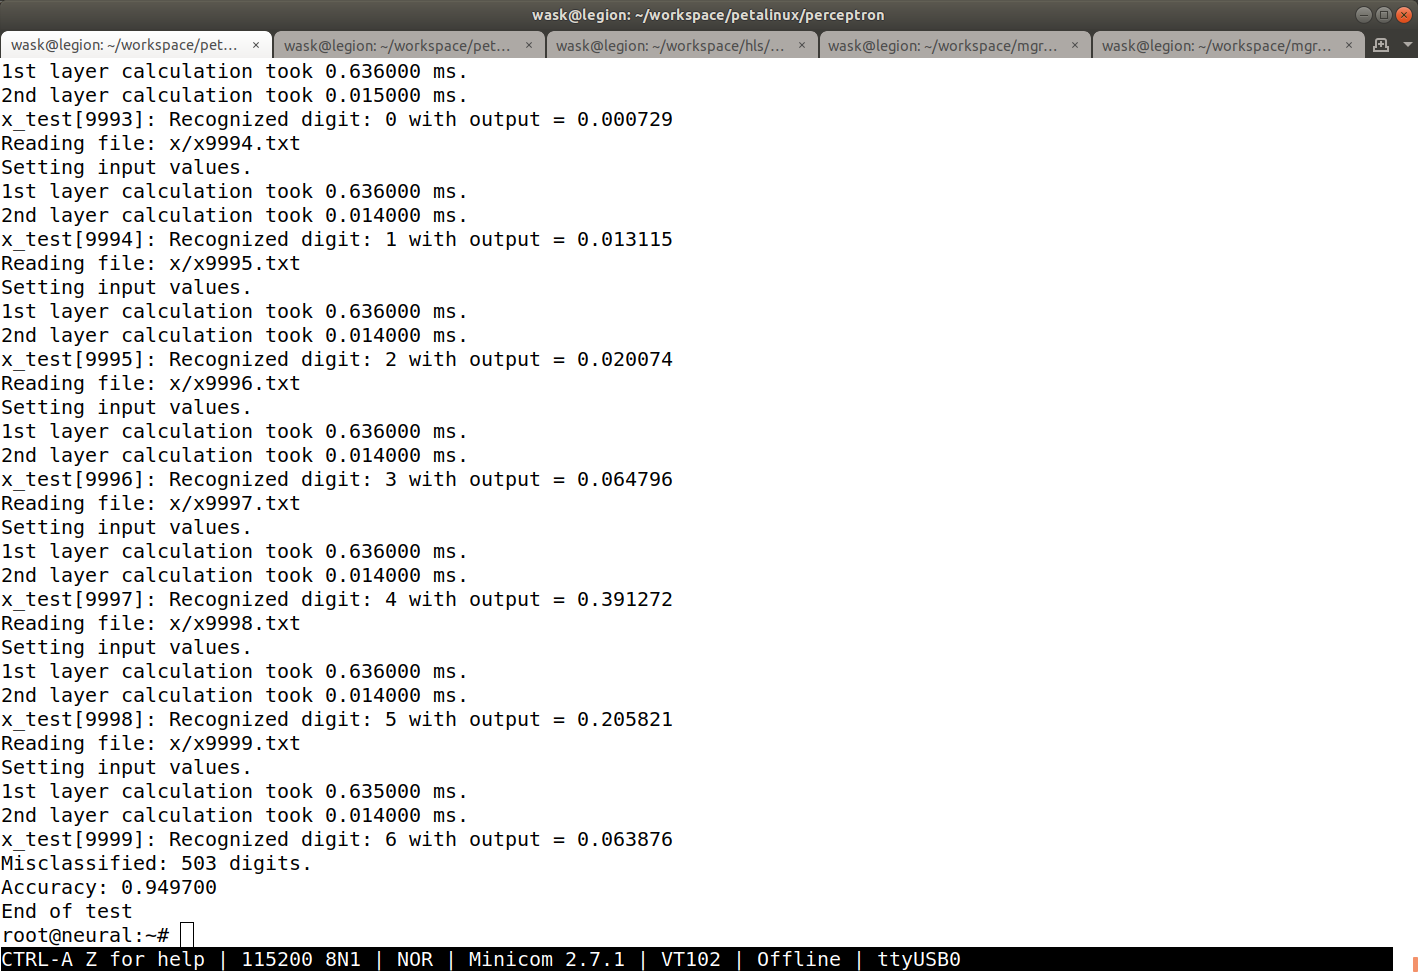
\includegraphics[width=\textwidth]{img/wynik1.png}
    \caption{Wynik testu uruchomionego na SBC Z-turn -- ANN z jedną warstwą ukrytą}
    \label{wynik1}
  \end{figure}


\subsubsection{Test klasyfikacji cyfr z użyciem kamery}

Następnym krokiem był test przeprowadzony w czasie rzeczywistym z użyciem kamery. Rozpoznawanie obiektów na obrazie w czasie rzeczywistym podzielono na 3 części:
\begin{itemize}
    \item detekcja kształtów przypominających cyfry i odrzucenie niewłaściwych obiektów
    \item przygotowanie obrazów do klasyfikacji (odpowiedni rozmiar obrazu i padding)
    \item klasyfikacja obrazów przy użyciu ANN
\end{itemize}

Pierwszą symulację wykonano na komputerze PC przy użyciu biblioteki OpenCV i pakietu \emph{keras}.
Ze względu na sporą ilość obliczeń początkowo zdecydowano się na zarejestrowanie obrazu oraz detekcję cyfr przy użyciu biblioteki OpenCV. 

Obraz był rejestrowany w rozdzielczości 640x480 pikseli przy użyciu funkcji \emph{cv2.VideoCapture(2)}. Następnym krokiem 
było przekształcenie barwy obrazu na skalę szarości, rozmycie obrazu oraz za pomocą funkcji \emph{cv2.adaptiveThreshold} 
przekształcenie w obraz binarny z odwróconymi kolorami. Istotne jest, żeby obraz zawierał białą cyfrę na czarnym tle, ponieważ takie obrazy były w zbiorze uczącym.  Następnie użyto funkcji \emph{cv2.findContours}, która zwraca współrzędne prostokątów, w które wpisane są kontury znalezione przez algorytm. Po wyeliminowaniu niewłaściwych konturów można przejść do przygotowania obrazów do klasyfikacji. 

\begin{figure}[!h]
    \centering
    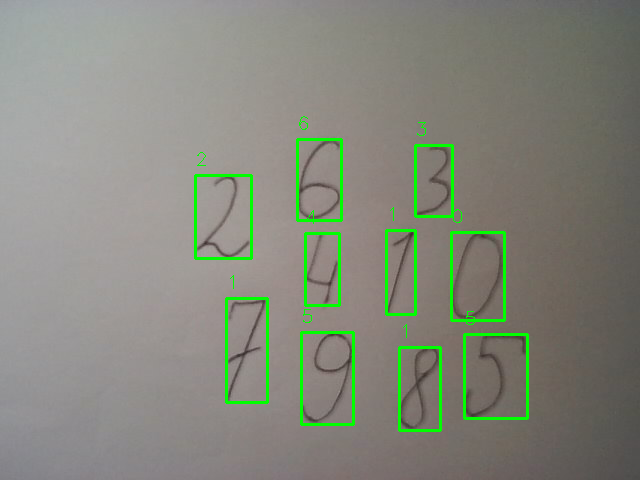
\includegraphics[width=\textwidth]{img/1hid-layer-pc-img.png}
    \caption{Ramka obrazu podczas testu ANN z jedną warstwą ukrytą uruchomionego na PC}
    \label{1hid-layer-pc-img}
  \end{figure}

Odpowiednio przycięty do rozmiaru 28x28 pikseli i wycentrowany obraz ręcznie pisanej cyfry może zostać poddany klasyfikacji za pomocą nauczonego wcześniej modelu ANN. W wyniku testu otrzymano wyniki przedstawione na Rys. \ref{1hid-layer-pc-img}. 

\begin{figure}[!h]
    \centering
    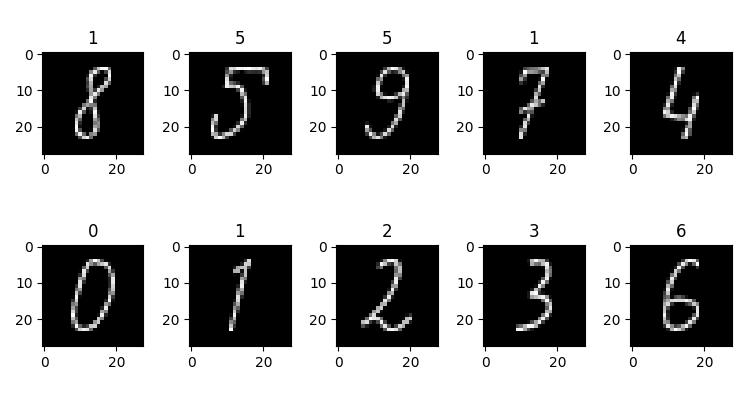
\includegraphics[width=\textwidth]{img/1hid-layer-pc-plot.png}
    \caption{Wynik testu ANN z jedną warstwą ukrytą uruchomionego na PC}
    \label{1hid-layer-pc-plot}
\end{figure}


Rysunek Rys. \ref{1hid-layer-pc-plot} zawiera znalezione na obrazie cyfry i wynik klasyfikacji (nad każdą z cyfr). Widać, że 3 z 10 cyfr zostały sklasyfikowane nieprawidłowo, co daje dokładność klasyfikacji sieci 70\%.

\subsubsection{Test na płytce Z-turn z użyciem kamery}

W teście na płytce Z-turn zastosowano metodę rejestrowania obrazu taką jak na komputerze PC, jednak do rozpoznania cyfr wykorzystano model sieci ANN zaimplementowany w układzie FPGA. Aby umożliwić użytkownikowi wyświetlanie obrazu w czasie rzeczywistym, wykorzystano pakiety \emph{pickle} i \emph{socket} do wysyłania kolejnych ramek obrazu przez protokół TCP (ang. \emph{Transmission Control Protocol}). Wynik testu przedstawiono na Rys. \ref{1hid-layer-zturn-img}.

\begin{figure}[!h]
    \centering
    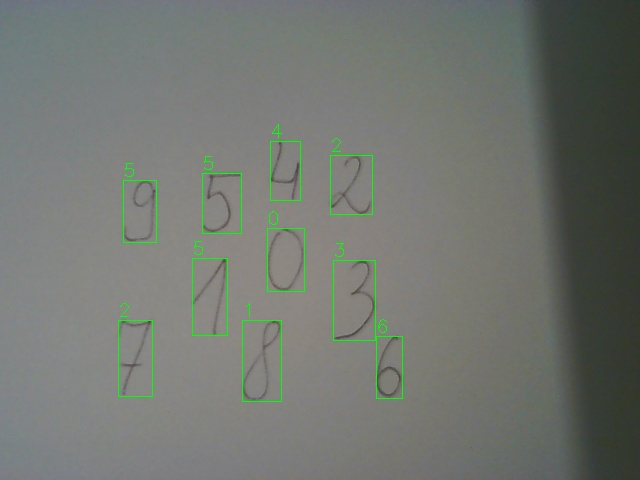
\includegraphics[width=\textwidth]{img/1hid-layer-zturn-img.jpg}
    \caption{Wynik testu ANN z jedną warstwą ukrytą uruchomionego na płytce Z-turn Board}
    \label{1hid-layer-zturn-img}
\end{figure}

Po otrzymaniu wyników pierwszego testu podjęto decyzję o modyfikacji modelu Sztucznej Sieci Neuronowej. Pierwszą zmianą było dodanie kolejnej warstwy ukrytej.

\subsection{Test modelu posiadającego dwie warstwy ukryte}

Dodano do istniejącego modelu kolejną warstwę ukrytą zawierającą 64 neurony. Po wykonaniu 50 epok otrzymano dokładność na poziomie 97,17\%. Wykres zmiany dokładności w kolejnych epokach przedstawiono na Rys. \ref{keras-accuracy2}.

\begin{figure}
    \centering
    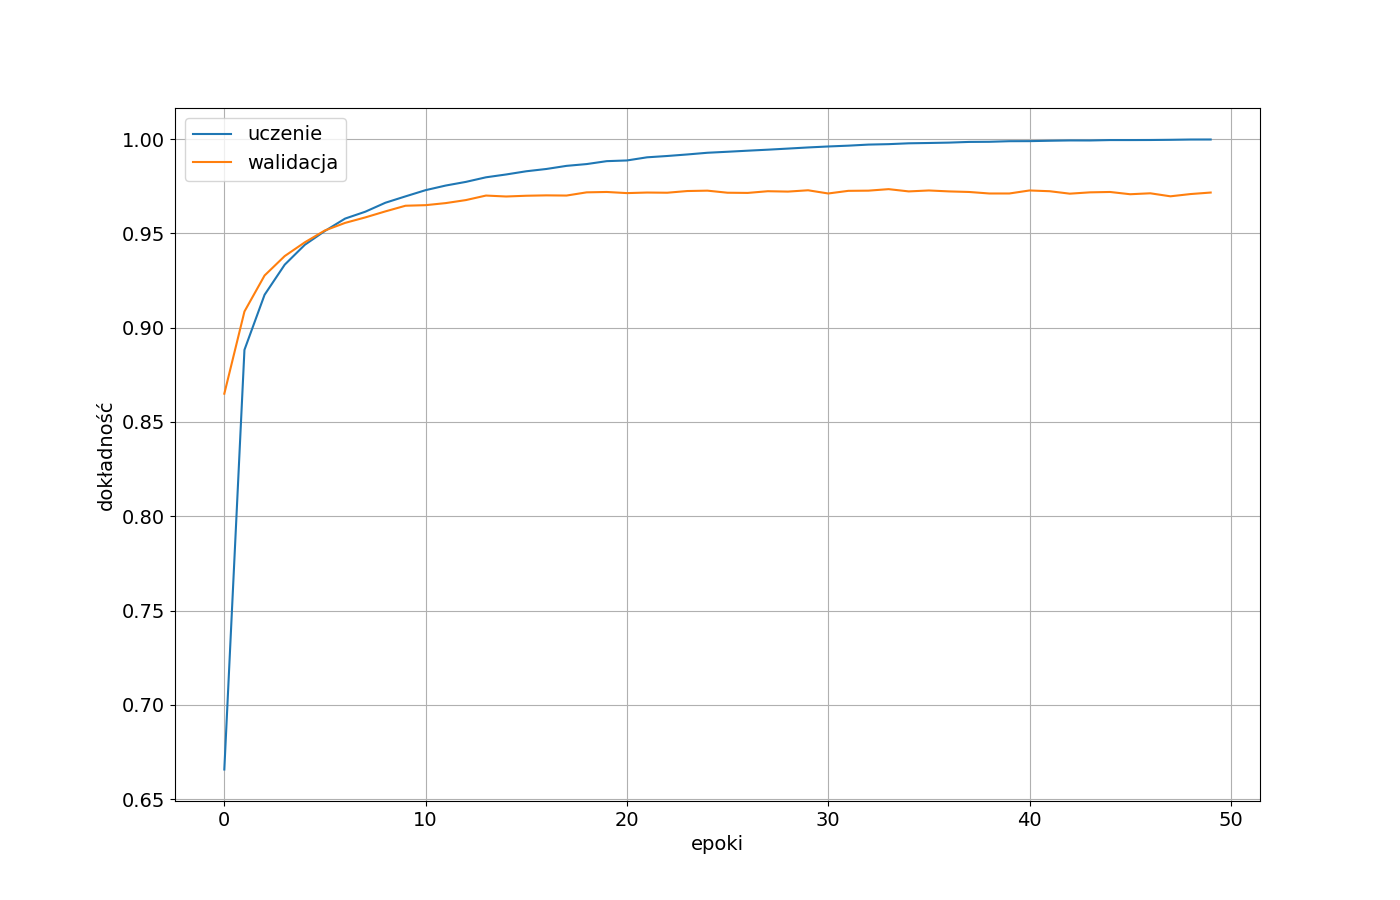
\includegraphics[width=\textwidth]{img/keras-accuracy2.png}
    \caption{Wykres zmian dokładności w kolejnych epokach -- ANN z dwoma warstwami ukrytymi}
    \label{keras-accuracy2}
  \end{figure}


\subsection{Implementacja modelu ANN w Vivado HLS}
  Parametry modelu sieci ANN stworzonego, nauczonego i przetestowanego w skrypcie Pythona z użyciem biblioteki keras są przekazywane do funkcji w Vivado HLS. Funkcja \emph{calcPerceptron()} jako argument przyjmuje następujące dane:
  \begin{itemize}
    \item dane wejściowe \emph{x} (obraz odręcznie pisanej cyfry)
    \item wagi sieci neuronowej \emph{w}
    \item biasy sieci neuronowej \emph{b}
    \item adres tablicy na dane wyjściowe sieci \emph{res}
    \item model sieci w postaci tablicy \emph{model} zawierającej:
    \begin{itemize}
      \item liczbę warstw sieci
      \item liczbę wejść sieci
      \item liczbę neuronów w każdej warstwie.
    \end{itemize}
  \end{itemize}

  Zmieniając wartości tablicy \emph{model}, użytkownik może zmieniać parametry sieci z poziomu aplikacji. Ograniczeniami są rozmiary tablic zawierających parametry sieci, które muszą być ustalone na etapie tworzenia projektu oraz ilość pamięci BRAM w układzie \emph{Zynq}.
   
Ponadto z poziomu aplikacji użytkownik ma możliwość ustawienia parametru progu przycinania sieci (ang. \emph{pruning threshold}). Dzięki temu możliwe jest wyeliminowanie redundantnych wag sieci i skrócenie obliczeń.

\subsection{Dostosowanie parametrów w implementacji HLS}

Implementacja umożliwiająca zmianę parametrów modelu sieci z poziomu aplikacji jest bardzo wygodnym rozwiązaniem, 
umożliwiającym szybkie przeprowadzenie testów dla różnych modeli sieci. Jednak zdefiniowanie w implementacji HLS parametrów 
sieci w postaci zmiennych, spowodowało znaczne ograniczenia w możliwościach optymalizacji. 

Pierwszym napotkanym problemem był brak możliwości pełnego rozwinięcia pętli przy użyciu dyrektywy:
\begin{verbatim}
  #pragma HLS UNROLL
\end{verbatim}
spowodowany zastosowaniem w zmiennej, będącej parametrem funkcji, w warunku zakończenia pętli. Rozwiązaniem było zastosowanie parametru rozwijania pętli równego 2.



%perfect loops i nie perfect ;)

% Perfect Loops
% Only the inner most loop has body (content).
% There is no logic specified between the loop statements.
% The loop bounds are constant.

% Semi-Perfect Loops
% Only the inner most loop has body (content)
% There is no logic specified between the loop statements.
% The outer most loop bound can be variable.

% In  the  following,  we  attempt  to  demonstrate  several  concepts.   First,  writing  efficienthigh-level synthesis code requires that the designer must understand hardware concepts likeunrolling and partitioning.  Second, the designer must be able to diagnose any throughputproblems, which requires substantial knowledge about both the application and the hardwareimplementation of that design.  Third, and most importantly, in order to achieve the bestresults – high performance and low-area – it is typically required to rewrite code in a mannerthat will create an efficient hardware architecture.  This is often very different than code thatwill create efficient software

% opisz jakie były ograniczenia 

Aby osiągnąć maksymalną akcelerację obliczeń i optymalizację zasobów zmieniono założenia projektu. Parametry modelu zostały ustalone na etapie implementacji bloku HLS. Ze względu na dużą dokładność klasyfikacji wybrano następujący model:

\begin{verbatim}
_________________________________________________________________
Layer (type)                 Output Shape              Param #   
=================================================================
flatten_1 (Flatten)          (None, 784)               0         
_________________________________________________________________
dense_1 (Dense)              (None, 16)                12560     
_________________________________________________________________
dense_2 (Dense)              (None, 10)                170       
=================================================================
Total params: 12,730
Trainable params: 12,730
Non-trainable params: 0
_________________________________________________________________
\end{verbatim}

W wyniku uczenia sieci otrzymano dokładność klasyfikacji na poziomie 94,14\%.

Wybrany model zaimplementowano w programie Vivado HLS. Ustalenie wartości liczby wejść i neuronów dało większe możliwości optymalizacji. 

Następnym problemem związanym z rozwijaniem pętli był komunikat Vivado HLS o braku możliwości wykonania operacji wczytania danych z jednej z tablic spowodowany posiadaniem tylko dwóch portów pamięci BRAM. Sugerowanym rozwiązaniem jest użycie innego bloku pamięci pozwalającego na równoległy odczyt dużej ilości danych lub partycjonowanie tablicy.

\begin{figure}[!h]
  \centering
  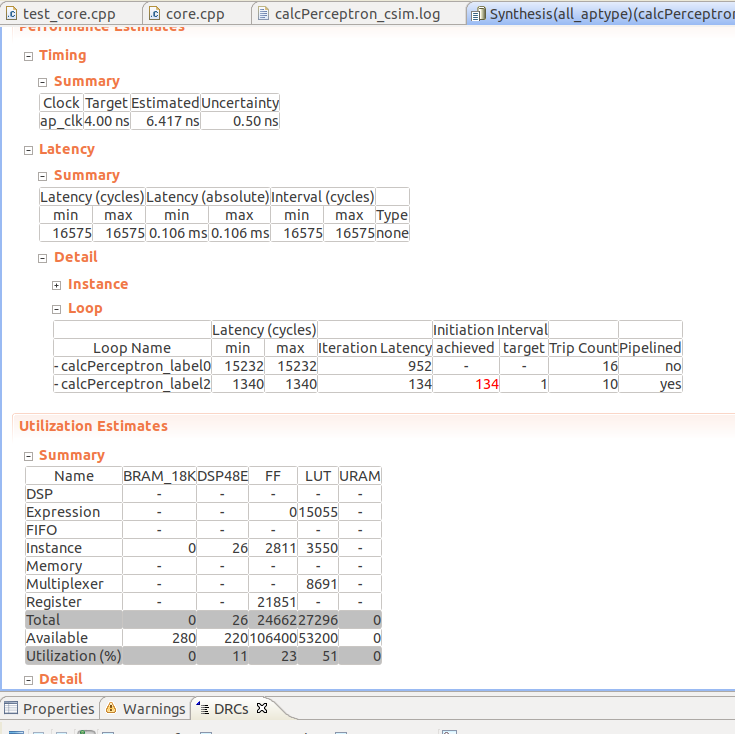
\includegraphics[width=\textwidth]{img/hls-report2.png}
  \caption{Raport po przeprowadzeniu syntezy w Vivado HLS -- drugie podejście}
  \label{hls-report2}
\end{figure}

\subsection{Arytmetyka stałoprzecinkowa}

Kolejną metodą optymalizacji kodu jest zastosowanie arytmetyki stałoprzecinkowej. Przy użyciu biblioteki \emph{<ap\_fixed.h>} zaimplementowano oddzielne typy dla każdej ze zmiennych reprezentujących parametry sieci. Po wykonaniu analizy raportu dla różnych konfiguracji typów stałoprzecinkowych okazało się, że wprowadzenie arytmetyki stałoprzecinkowej w tym projekcie daje duże zużycie zasobów (ponad 100\%), przy nieznacznym spadku opóźnień. W związku z tym zdecydowano się na wykorzystanie typu zmiennoprzecinkowego.


\subsection{Porównanie czasu wykonania różnych implementacji}

Średni wynik obliczenia wyjścia sieci neurononwej przy użyciu pakietu keras na komputerze PC to 0.167040 $\mu$s. W przypadku implementacji w układzie FPGA było to 0.470000 $\mu$s. daje to współczynnik akceleracji obliczeń ok. 2.81 co jest dobrym wynikiem, biorąc pod uwagę ograniczenia w optymalizacji kodu w narzędziu Vivado HLS.
